% ------------------------------------------------------------%
% 2015-2021 - Emerson Ribeiro de Mello <mello@ifsc.edu.br>
% ------------------------------------------------------------%
% Sets aspect ratio to 4:3, and frame size to 128 mm by 96 mm
\documentclass[aspectratio=169]{beamer}
% Sets aspect ratio to 16:9, and frame size to 160 mm by 90 mm.
% \documentclass[aspectratio=169]{beamer}
% Sets aspect ratio to 16:10, and frame size to 160 mm by 100 mm.
% \documentclass[aspectratio=1610]{beamer}
\usepackage[dvipsnames]{xcolor}
\usepackage{colortbl}
\usepackage{makecell}
\usepackage{multicol}
\usepackage{pifont}

\definecolor{DarkCyan}{HTML}{119DA4}
\definecolor{Asparagus}{HTML}{6DA34D}
\definecolor{CambridgeBlue}{HTML}{8FBC94}
\definecolor{TeaGreen}{HTML}{C5E99B}
\definecolor{Saphire}{HTML}{4059AD}



% -------------------------------------------------%
%  Package options
% -------------------------------------------------%
%  002625, EEE5E9, 0D1821, ADF7B6, B6C454
% textbgcolor   - frametitle background color. default: 0d4f4d
% textfgcolor   - frametitle foreground color. default: ffffff
% slidebgcolor  - slide background color. default: eef1ec
% slidefgcolor  - slide text foreground color. default: 000000
% authorfgcolor - author, institute and date color. default: 000000
% itemsep - space between items (itemize, enumerate). default: 7pt
\usepackage[textbgcolor=344966,textfgcolor=ffffff,slidebgcolor=EEE5E9,itemsep=7pt]{../0-ifscyan-modelo/beamerthemeifscyan}
% -------------------------------------------------%

% A good place to get some colors
% https://material.io/resources/color/#!/?view.left=0&view.right=0&primary.color=0d4f4d
% cyan: #0D4F4D, light: #417b79,  dark: #002625
% IFSC green: normal: #32A041, light: #69d26f, dark: #007013
% IFSC red: normal: #C8191E, light: #ff5747, dark: #8f0000 
% Other colors for textbgcolor
% purple 4527a0, blue 0d47a1, grey 546e7a, redwine 880e4f, brown 6d4c41, yelllow (bg=#fbc02d, fg=000000)

% Logo
\pgfdeclareimage[height=.3\paperheight]{ifpilogo}{../0-ifscyan-modelo/figs/Logo-IFPI-Vertical.png}

\AtBeginSection[]{
  \begin{frame}
  \vfill
  \centering
  \begin{beamercolorbox}[sep=8pt,center,shadow=true,rounded=true]{title}
    \usebeamerfont{title}\insertsectionhead\par%
  \end{beamercolorbox}
  \vfill
  \end{frame}
}

% -------------------------------------------------%
%              Título 
% -------------------------------------------------%
\title{Matemática Computacional}
\subtitle{Conjuntos}
\author{Prof. Rogério Figueredo de Sousa}
\institute{%
\href{rogerio.sousa@ifpi.edu.br}{rogerio.sousa@ifpi.edu.br}%
}%
\date{05/07/2024}
% -------------------------------------------------%

% -------------------------------------------------%
%  Início do documento 
% -------------------------------------------------%
\begin{document}

\begin{frame}[plain]
    \titlepage
\end{frame}

%\begin{frame}[plain, noframenumbering]{Licenciamento}
%    \licenciamentoLivre
%\end{frame}

%\begin{frame}[plain, noframenumbering]{Sumário}
%   \tableofcontents
%\end{frame}


\jsonp
\lstset{
    numbers=none,
    escapeinside={\%*}{*)},
}

%1
\begin{frame}{Conjuntos}

    Conjunto não se define formalmente. Usa-se uma ideia intuitiva de que se trata de uma coleção de objetos, logo, informalmente, um conjunto é uma coleção desordenada de zero ou mais objetos, denominados elementos do conjunto. Dizemos que um conjunto contém seus elementos.

    \begin{itemize}
        \item Esses objetos de um conjunto possuem alguma propriedade em comum.
        \item Em geral, trata-se de uma estrutura discreta, usada para construir outras estruturas;
        \item O propósito fundamental é o de agrupar elementos.
    \end{itemize}

\end{frame}

%2
\begin{frame}{Conjuntos}
    Notação: Indicamos um conjunto, em geral, com uma letra maiúscula e um elemento com letra minúscula.

    \begin{itemize}
        \item Se A é um conjunto e x pertence a A, esse fato é denotado por: $x \in A$.
        \item Se, por outro lado, tivermos que x não pertence ao conjunto A, escrevemos: $x \notin A$.
    \end{itemize}

    \vspace{2mm}
    Usamos chaves para indicar um conjunto.
    \begin{itemize}
        \item Se $A = \{azul, verde, branco\}$, então $verde \in A$ e $preto \notin A$.
        \item Os elementos em um conjunto não tem nenhuma ordem, de modo que $\{azul, verde, branco\}$ é o mesmo que $\{branco, azul, verde\}$.
    \end{itemize}    

\end{frame}


%3
\begin{frame}{Conjuntos}
    Dois conjuntos são \textbf{iguais} se contêm os mesmos elementos. Ou seja,

    \[ A = B ~ significa ~ (\forall x)[ x \in A \rightarrow x \in B \land (x \in B \rightarrow x \in A)] \]

    \begin{itemize}
        \item Ao descrever um conjunto particular, temos que identificar seus elementos.
        \item Para um \textbf{conjunto finito} (com n elementos para $n > 0$), isso é feito listando-se todos os seus elementos.
        \item Para um \textbf{conjunto infinito}, podemos indicar a forma geral listando os primeiros elementos.
    \end{itemize} 

\end{frame}

%4
\begin{frame}{Conjuntos}
    Conjunto infinito: exemplos:

    \begin{itemize}
        \item $A=\{2,4,6,...\}$
        \item $B=\{0,1,2,3,4,...\}$
        \item $C=\{2,4,8,16,..\}$
    \end{itemize}

    \vspace{4mm}
Ou podemos representar por uma relação de recorrência. 

\begin{itemize}
    \item $ 2 \in A $
    \item se $ n \in A, $ então $ n + 2 \in A $
\end{itemize}

\vspace{2mm}

Temos, $A=\{2,4,6,...\}$

\end{frame}


%5
\begin{frame}{Conjuntos}
    Conjunto infinito: exemplos:

    \begin{itemize}
        \item $0 \in B $
        \item se $n \in B$, então $n + 1 \in B$
    \end{itemize}
    
    \vspace{2mm}
Temos, $B=\{0,1,2,...\}$

\vspace{4mm}
\begin{itemize}
    \item $2 \in C $
    \item se $n \in C$, então $2n \in C$
\end{itemize}

\vspace{2mm}
Temos, $C=\{2,4,8,16...\}$

\end{frame}

%6
\begin{frame}{Conjuntos}
    A \textbf{descrição} um conjunto pode ser feita de várias maneiras, conforme segue.
  
    \begin{enumerate}[a)]
        \item Enumerando seus elementos, entre chaves:
    \end{enumerate}

    \vspace{4mm}

Exemplos:

\begin{enumerate}
    \item $V = \{ a, e, i, o, u\}$
    \item $I = \{1, 3, 5, 7, 9, ...\}$
    \item $D = \{0, 1, 2, 3, ..., 9\}$
    \item $Q = \{0, 1, 4, 9, 25, 36, ...\}$
    \item $P = \{2, 3, 5, 7, 11, ...\}$
\end{enumerate}

\end{frame}

%7
\begin{frame}{Conjuntos}
    \begin{enumerate}[b)]
        \item Quando conhecemos uma certa propriedade característica de seus elementos:
    \end{enumerate}
    
    \vspace{4mm}

Escrevemos $A = \{ x \mid P(x) \}$, x tem um predicado P. Ou seja,

\[ A = \{x \mid P(x)\} ~ significa ~ (\forall x)[(x \in S \rightarrow P(x)) \land (P(x) \rightarrow x \in S)] \]

\vspace{4mm}
Exemplo:

\vspace{2mm}
$A= \{ x \vert x ~ \acute{e} ~ um ~ inteiro ~ positivo ~ par \}$

\vspace{4mm}
``O conjunto de todos os x tais que x é um inteiro positivo par''

\end{frame}

%8
\begin{frame}{Conjuntos}
    Exemplos:
    \vspace{4mm}

    \begin{enumerate}
        \item $L = \{x \vert x ~ \acute{e} ~ aluno ~ do ~ primeiro ~ semestre ~ do ~ Curso ~ de ~ ADS\}$
        \item $D = \{x \vert x ~ \acute{e} ~ inteiro ~ positivo ~ menor ~ que ~ 10 \}$
        \item $N = \{x|x ~ \acute{e} ~ n\acute{u}mero ~ natural ~ e ~ 4 < x < 3500\}$
        \item $M = \{x|x ~ \acute{e} ~ m\acute{u}ltiplo ~ de ~ 5\}$
        \item $P = \{x|x ~ \acute{e} ~ um ~ n\acute{u}mero ~ real\}$
    \end{enumerate}

\end{frame}

%9
\begin{frame}{Conjuntos}
    Exemplo:
    \vspace{4mm}
    
    Seja um conjunto A dado por:

    \[ A = \{x | (\exists y)(y \in \{0, 1, 2\} ~ e ~ x = y^3\} \]

    \begin{itemize}
        \item Esse conjunto é da forma $A=\{x|P(x)\}$.
        \item Encontra-se cada elemento de A atribuindo-se a y cada um dos valores e elevando-os ao cubo.
        \item Então $A = \{0, 1, 8\}$
    \end{itemize}
\end{frame}

%10
\begin{frame}{Conjuntos}
    \begin{enumerate}[c)]
        \item Por uma relação de recorrência:
    \end{enumerate}

    \vspace{4mm}
    Exemplos:

    \begin{enumerate}
        \item Sequência de Fibonacci
        
        \begin{itemize}
            \item $F(1) = 1$
            \item $F(2) = 1$
            \item $F(n) = F(n-1) + F(n-2),$
        \end{itemize}

        \vspace{4mm}
        \item 
        
        \begin{itemize}
            \item $1 \in S$
            \item Se $x \in S$, então $X + 2 \in S$
        \end{itemize}
    \end{enumerate}
    

\end{frame}

%11
\begin{frame}{Conjuntos}
    É conveniente usarmos uma notação padrão para determinados conjuntos, de modo que se possa se referir mais facilmente a eles.

    \vspace{4mm}

    \begin{multicols}{2}
        \begin{description}
            \item[$\mathbb{N} =$] Números naturais
            \item[$\mathbb{Z} =$] Números inteiros
            \item[$\mathbb{R} =$] Números reais
            \item[$\mathbb{Q} =$] Números racionais
            \item[$\mathbb{I} =$] Números Irracionais 
        \end{description}
        
        \columnbreak

        \begin{center}
            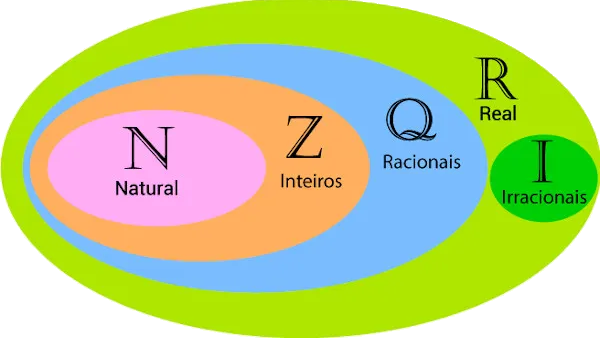
\includegraphics[width=\linewidth]{figs/conjuntos.png}
        \end{center}
    \end{multicols}
    
\end{frame}


%12
\begin{frame}{Conjuntos - Exercícios}
    Exercício 1: Julgue se os conjuntos são finitos ou infinitos:
    \vspace{4mm}
\begin{enumerate}
    \item Conjunto das letras do alfabeto;
    \item $P = \{y | y = 2x ~ e ~ x \in \mathbb{N} \}$
    \item $M = \{x \in \mathbb{N} | x > 0 ~ e ~ x < 6\}$
    \item O conjunto do números naturais.
\end{enumerate}    
\end{frame}

%13
\begin{frame}{Conjuntos - Exercícios}
    Exercício 2: Descreva cada um dos conjuntos a seguir listando seus elementos:
    \vspace{4mm}
\begin{enumerate}
    \item $A=\{x|x ~ \acute{e} ~ um ~ inteiro ~ e ~ 3 < x < 8\}$
    \item $B=\{x|x ~ \acute{e} ~ um ~ m\hat{e}s ~ com ~ exatamente ~ 30 ~ dias\}$
    \item $C=\{x|x ~ \acute{e} ~ a ~ capital ~ do ~ Brasil\}$
    \item $D=\{x|(\exists y)(y \in \{0,1,2\} ~ e ~ x = y^3)\}$
    \item $E=\{x|x \in \mathbb{N} ~ e ~ (\exists y)(y \in \mathbb{N} ~ e ~ x \leq y)\}$
    \item $F=\{x|x \in \mathbb{N} ~ e ~ (\forall y)(y \in \mathbb{N} ~ \rightarrow ~ x \leq y)\}$
    \item $A = \{x | x \in \mathbb{N} ~ e ~ (\forall y)(y \in \{2, 3, 4, 5\}) \rightarrow x \geq y\}.$
    \item $B = \{x | (\exists y)(\exists z)(y \in \{1,2\} ~ e ~ z \in \{2,3\} ~ e ~ x=y+z)\}$
\end{enumerate}    
\end{frame}

%14
\begin{frame}{Conjuntos - Exercícios}
    Exercício 3: Descreva cada um dos conjuntos a seguir através de uma relação de recorrência.
    \vspace{4mm}
\begin{enumerate}
    \item $A=\{2,4,16,256,...\}$
    \item $B=\{1,4,9,16,...\}$
    \item $C=\{1,3,9,27,...\}$
    \item $D=\{2,3,5,7,11,...\}$
\end{enumerate}    
\end{frame}

%15
\begin{frame}{Conjuntos}
    \textbf{Conjuntos importantes:}
    \vspace{4mm}

\begin{enumerate}
    \item Conjunto Conjunto Unitário: é um conjunto que possui um único elemento.
 
    \vspace{2mm}
    Exemplos:
    \begin{enumerate}[i)]
        \item Conjunto das soluções da equação $5x + 4 = 19$.
        \item Conjunto de todos os números que são pares e primos simultaneamente.
    \end{enumerate}

    \item Conjunto vazio: é um conjunto que não possui elemento algum. Notação: $A = \{ \} = \emptyset $
    
    \vspace{2mm}
    Exemplos:
    \begin{enumerate}[i)]
        \item Conjunto dos brasileiros com mais de 400 anos.
        \item $\{x|x ~ \acute{e} ~ \acute{i}mpar ~ e ~ m\acute{u}ltiplo ~ de ~ 2\}$
    \end{enumerate}
\end{enumerate}   

\end{frame}

%16
\begin{frame}{Conjuntos}
    \begin{enumerate}[3]
        \item Conjuntos Numéricos:
        
        \begin{enumerate}[a]
            \item Naturais: $\mathbb{N} = \{0,1,2,3, ... \}$
            \item Inteiros: $\mathbb{Z} = \{..., -3,-2,-1,0,1,2,3, ... \}$
            \item Racionais: $\mathbb{Q} = \{p / q | p \in \mathbb{Z}, q \in \mathbb{Z},q \neq 0 \}$
            \item Irracionais ($\mathbb{I}$): \textit{\{x|x não pode ser escrito na forma de fração, com p e q inteiros\}}
            \item Reais($\mathbb{R}$): é a reunião dos racionais com irracionais.
            \item Complexos ($\mathbb{C}$): tem a forma $a + bi$, com $i^2=-1$
        \end{enumerate}
    \end{enumerate}
\end{frame}

%17
\begin{frame}{subconjuntos}
    Um conjunto \textbf{A é subconjunto de um conjunto B} se, e somente se, \textbf{todo elemento de A também é elemento de B}.

    \vspace{4mm}
    Dizemos neste caso que \textbf{A está contido em B}, ou ainda, que \textbf{B contém A}.

    \[ A \subseteq  B \leftrightarrow (\forall x)(x \in A \rightarrow x \in B )\]

    Se existe

    \[ b \in B ~ e ~ b \notin A, ~ ent\tilde{a}o ~ A \subset B \]

    \vspace{4mm}
    Neste caso A é um subconjunto próprio de B.

    \vspace{4mm} 
    OBS.: $A \subseteq A$ e $ \emptyset \subseteq  A$
\end{frame}


%18
\begin{frame}{subconjuntos}
    \textbf{Exemplos:}
    \vspace{4mm}

    \begin{enumerate}
        \item Para $A=\{2, 3, 5, 12\}$ e $B=\{2, 3, 4, 5, 9, 12\}$, todo elemento de A é, também, elemento de B.
        \begin{itemize}
            \item A é um subconjunto de B. ($A \subseteq B$)
            \item A é também subconjunto próprio de B. ($A \subset B$)
        \end{itemize}

        \item Sejam $A=\{1, 7, 9, 15\}$, $B=\{7, 9\}$ e $C=\{7, 9, 15,20\}$, então as seguintes proposições são verdadeiras (entre outras):
        \begin{multicols}{2}
            \begin{itemize}
                \item $B \subseteq  C$
                \item $B \subseteq  A$
                \item $B \subset  C$
                \item $A \nsubseteq C$
                \item $15 \in C$
                \item $\{7, 9\} \subseteq B$
                \item $\{7\} \subset A$
                \item $ \emptyset \subseteq C$
            \end{itemize}
    \end{multicols}
    \end{enumerate}
    
\end{frame}

%19
\begin{frame}{subconjuntos}
    \textbf{Exemplos:}
    \vspace{4mm}

    \begin{itemize}
        \item $\mathbb{N} \subset \mathbb{Z}$.
        \begin{itemize}
            \item Todo elemento de $\mathbb{N}$ é também um elemento de $\mathbb{Z}$.
            \item Porém, nem todo inteiro está presente em $\mathbb{N}$.
            \item Contra-exemplo: inteiros negativos. 
        \end{itemize}

        \item $S \subset \mathbb{N}$, onde $S = \{ x | x ~ \acute{e} ~ primo\}$:
        \begin{itemize}
            \item Todo número primo é também um número natural.
            \item Porém, nem todo natural é um número primo.
            \item Contra-exemplos: naturais pares (exceto 2).
        \end{itemize}
    \end{itemize}
    
\end{frame}

%20
\begin{frame}{subconjuntos}
    \textbf{Exercício:}
    \vspace{4mm}

    Sejam $A = \{x | x \in \mathbb{N} ~ e ~ x \geq 5\}$, $B = \{10, 12, 16, 20\}$ e $C = \{x | (\exists y)(y \in \mathbb{N} ~ e ~ x = 2y)\}$

    Quais das proposições abaixo são verdadeiras:
    
    \begin{multicols}{2}
        \begin{itemize}
            \item $B \subseteq C$
            \item $B \subset A$
            \item $A \subseteq C$
            \item $26 \in C$
            \item $\{11, 12, 13\} \subseteq A$
            \item $\{11, 12, 13\} \subset C$
            \item $\{12\} \in B$
            \item $\{12\} \subseteq B$
            \item $\{x | x \in \mathbb{N} ~ e ~ x < 20\} \nsubseteq B$
            \item $5 \subseteq A$
            \item $\{\emptyset\} \subseteq B$
            \item $\emptyset \notin A$
        \end{itemize}
    \end{multicols}
\end{frame}

%20
\begin{frame}{subconjuntos}
    \textbf{Exercício:}
    \vspace{4mm}
    
    Sejam: 
    
    \[A = \{x | x \in \mathbb{R} ~ e ~ x^2 - 4x + 3 = 0\}\]

e

    \[B = \{x | x \in \mathbb{N} ~ e ~ 1 \leq x \leq 4\}\]
    \vspace{4mm}
Prove que $A \subset B.$

\end{frame}

%20
\begin{frame}{subconjuntos}
   \textbf{ Conjuntos iguais:} dois conjuntos são iguais se todo elemento de A pertence a B e vice-versa, ou seja eles possuem os mesmos elementos.

   \vspace{4mm}

   Formalmente,

   \[ A = B \leftrightarrow \forall x (x \in A \leftrightarrow x \in B) \]

   Exemplos:

%    \vspace{4mm}

    \begin{itemize}
        \item $ A = \{1,3,5\}$ e $ B = \{5,3,1\}$. $A = B$
        \item $ A = \{1,3,5\}$ e $ B = \{1,1,5,5,5,5,3\}$. $A = B$
        \item $ A = \{1,3,5\}$, $ B = \{1,1,5,5,5,5,3\}$ e C = $\{3,1,5\}$. $A = B = C$
        \item $ A = \{1,3,5\}$, $ B = \{1,5,\}$ e $C = \{5,5,5,3,3,1\}$. $A = B$, $A \neq B$.
        \item $ A = \{1,3,5\}$ e $ B = \{1,5,1,5,1,5\}$. $A \neq B$
    \end{itemize}
\end{frame}


%21
\begin{frame}{subconjuntos}
    \textbf{ Exercício:} Sejam

    \[ A = \{x|x \in \mathbb{N} ~ e ~ x^2 < 15\} \]
    e
    
    \[ B = \{x|x \in \mathbb{N} ~ e ~ 2x < 7 \} \]

    Prove que $A = B.$
 
 \end{frame}

 %22
 \begin{frame}{subconjuntos}
    \textbf{Conjuntos de Conjuntos}
    \begin{itemize}
        \item Para um conjunto S, podemos formar um novo conjunto cujos elementos são subconjuntos de S.
        \begin{itemize}
            \item Esse novo conjunto é chamado de \textbf{conjunto das partes} de S e é denotado por $\wp(S) $
            \item Para $S=\{0,1\}$, $\wp(S) = \{\emptyset, \{0\}, \{1\}, \{0,1\}\}.$
            \item Os elementos do conjunto das partes de S são conjuntos.
            \item Para qualquer conjunto S, $\wp(S)$ sempre tem, pelo menos $\emptyset$ e S como elementos, já que é sempre verdade que $\emptyset \subseteq S$ e $S \subseteq S.$
            \item Para encontrar $\wp(S)$, comece com $\emptyset$, depois coloque os conjuntos formados por 1 elemento de S, depois ao formados por 2 elementos de S, por 3 e assim por diante, até o próprio S.
        \end{itemize}
    \end{itemize}
\end{frame}

%23
\begin{frame}{subconjuntos}
    \textbf{Exercício:} 
    
    \begin{enumerate}
        \item Para $A=\{1,2,3\}$, qual é o $\wp(A)$?
        \vspace{4mm}
        \item Se S tem \textit{n} elementos, então $\wp(A)$ tem quantos elementos?
    \end{enumerate}
        
\end{frame}

%24
\begin{frame}{subconjuntos}
    \textbf{Partição de um Conjunto - Definição}: Uma partição de um conjunto A é um conjunto de subconjuntos não-vazios, disjuntos entre si, cuja união é igual a A.
    
    \vspace{4mm}
    \textbf{Requisitos:}

    \begin{itemize}
        \item Cada subconjunto na partição deve ser não-vazio.
        \item Os subconjuntos devem ser mutuamente disjuntos (não têm elementos em comum).
        \item A união de todos os subconjuntos na partição deve ser igual ao conjunto original A.
    \end{itemize}
    
    \vspace{4mm}
    Exemplo: 

    \vspace{2mm}

    Para $A=\{1,2,3,4\}$, uma partição possível de A é $\mathcal{P}(A) = \{\{1,2\},\{3,4\}\}$.
        
\end{frame}

%25
\begin{frame}{subconjuntos}
    \textbf{Questão: }
    \noindent
Sobre o conjunto $A = \{1, 2, 3, 4\}$, considere as afirmativas a seguir.

\begin{enumerate}
    \item $\mathcal{P}(A) = \{\emptyset, \{2, 3, 4\}\}$ é uma partição de $A$.
    \item $\mathcal{P}(A) = \{\emptyset, \{1, 2, 3\}, \{3, 4\}\}$ é uma partição de $A$.
    \item $\mathcal{P}(A) = \{\{1, 2\}, \{3, 4\}\}$ é uma partição de $A$.
    \item $\mathcal{P}(A) = \{\{1\}, \{2\}, \{3\}, \{4\}\}$ é uma partição de $A$.
\end{enumerate}

\noindent
Assinale a alternativa correta.

\begin{enumerate}[a)]
    \item Somente as afirmativas I e II são corretas;
    \item Somente as afirmativas I e IV são corretas;
    \item Somente as afirmativas III e IV são corretas;
    \item Somente as afirmativas I, II e III são corretas;
    \item Somente as afirmativas II, III e IV são corretas;
\end{enumerate}
\end{frame}

%26
\begin{frame}{subconjuntos}
    \textbf{Definição(Cardinalidade):} Seja A um conjunto. Se existem exatamente n elementos distintos em A, com $n \geq 0$, então dizemos que A é um conjunto finito e que n é a cardinalidade de A.

    \vspace{4mm}
\textbf{OBS.:} A cardinalidade de A é denotada por $|A|$.

\vspace{4mm}

\begin{enumerate}
    \item $A = \{x | x ~ \acute{e} ~ inteiro ~ \acute{i}mpar ~ e ~ x < 10\}$. Logo, $|A| = 5$.
    \item $B = \{x | x ~ \acute{e}  ~ uma ~ letra ~ do ~ alfabeto\}$. Logo, $|B|= 26$.
    \item $P = \{x | x ~ \acute{e} ~ primo ~ e ~ x < 30\}$. Logo, $|P| = 10$.
    \item $C = \emptyset$ . Como o conjunto vazio não possui elementos, Então $|\emptyset | = 0$.
\end{enumerate}
\end{frame}

%29
\begin{frame}{Operações em Conjuntos}
\begin{itemize}
    \item A maior parte das operações que envolvem números podem ser efetuadas também em conjuntos.
    \item Dado um conjunto S, podemos definir operações no conjunto $\wp(S)$.
    \begin{itemize}
        \item S, nesse caso, é chamado de \textbf{conjunto universo}, que define o contexto dos objetos em discussão.
        \item Se $S = \mathbb{Z}$, então os subconjuntos conterão apenas inteiros.
    \end{itemize}
    \item Operação unária e binária
    \begin{itemize}
        \item Unária: quando age em apenas um elemento do conjunto (por exemplo, uma negação de um elemento).
        \item Binária: quando acontece em dois inteiros do conjunto (por exemplo, uma subtração).
    \end{itemize}
\end{itemize}
\end{frame}

\begin{frame}{Operações em Conjuntos}
    \textbf{União:} Dados os conjuntos A e B chama-se união ou reunião de A e B, denotada por $A \cup B$, ao conjunto formado pelos elementos que pertencem a A ou a B.
    
    \vspace{4mm}
    Formalmente:

    \[A \cup B = \{x | x \in A ~ \boldsymbol{ou} ~ x \in B \}\]

    \textbf{Exemplo:}

    Sejam $A = \{1, 2, 4\}$ e $B = \{1, 3, 5\}$.

    $A \cup B = \{1, 2, 4\} \cup \{1, 3, 5\}$

    $A \cup B = \{1, 2, 3, 4, 5\}$

\end{frame}


\begin{frame}{Operações em Conjuntos}
    \textbf{Interseção:} Dados os conjuntos A e B a interseção de A e B, denotada por $A \cap B$, é o conjunto formado pelos elementos que pertencem a A e a B.
    
    \vspace{4mm}
    Formalmente:

    \[A \cap B = \{x | x \in A ~ \mathbf{e} ~ x \in B \}\]

    \textbf{Exemplo:}

    Sejam $A = \{1, 2, 4\}$ e $B = \{1, 3, 5\}$.

    $A \cap B = \{1, 2, 4\} \cap \{1, 3, 5\}$
    
    $A \cap B = \{1\}$

\end{frame}


\begin{frame}{Operações em Conjuntos}
  \textbf{  Conjuntos Disjuntos}: Dois conjuntos A e B são disjuntos se $A \cap B = \emptyset $.
    \vspace{4mm}
  \textbf{Exemplo:}

Sejam $A = \{1, 2, 3, 4\}$ e $B = \{5, 6, 7, 8\}$.

$A \cap B$ = elementos em comum entre A e B

$A\cap B=\emptyset$

Logo, A e B são disjuntos.
\end{frame}

\begin{frame}{Operações em Conjuntos}
    \textbf{Diferença: } Dados os conjuntos A e B. A diferença $A - B$ ou $A \backslash B$ contém os elementos que estão em A mas não estão em B.

    \vspace{4mm}
    Formalmente:

    \[ A - B = \{ x | x \in A \wedge x \notin B \} \]

    \textbf{Exemplo:}

    Sejam $A = \{a, b, c, d\}$ e $B = \{c, d, e, f, g\}$.

    $A \backslash B = \{a, b\}$

\end{frame}

\begin{frame}{Operações em Conjuntos}
\begin{figure}
    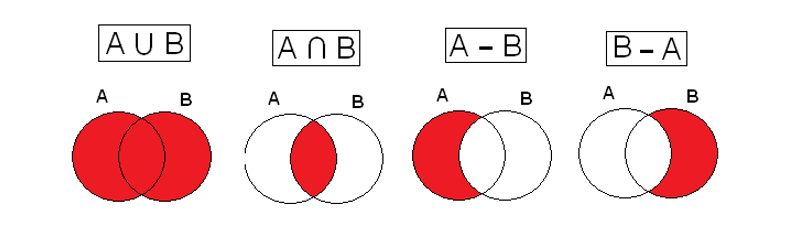
\includegraphics[width=0.9\textwidth]{./figs/operacoes.png}
\end{figure}
\end{frame}

\begin{frame}{Operações em Conjuntos}
    \textbf{Complementar: } Dados os conjuntos A e U(universo). O complementar de A em relação a U é o conjunto formado pela diferença $U - A$.

    \vspace{4mm}
    Formalmente:

    \[  A' = \{ x | x \in U ~ e ~ x \notin A \} \]

    \textbf{Exemplos:}

    \begin{enumerate}
        \item Seja $A = \{a, e, i, o, u\}$, onde o conjunto U são as letras do alfabeto.
    
        $A' = \{b, c, d, f, g, h, j, k, l, m, n, p, q, r, s, t, v, w, x, y, z\}$
    
        \item Seja $A = \{ x | x > 10\} $ e $U = \mathbb{Z}^+$
        
        $A' = \{1,2,3,4,5,6,7,8,9,10 \}$
    \end{enumerate}

\end{frame}

\begin{frame}{Exercícios}

    Sejam
\[ A = \{x | x ~ \acute{e} ~ um ~ inteiro ~ n\tilde{a}o - negativo ~ par \} \]
\[ B = \{x | (\exists y) (y \in \mathbb{N} ~ e ~ x = 2y + 1 )\} \]
\[ C = \{x|(\exists y)(y \in \mathbb{N} ~ e ~ x = 4y)\} \]

Julgue a veracidade de cada alternativa:

\begin{enumerate}[a)]
    \item $A \cup B$
    \item $A = B$
    \item $ C \subset A$
    \item $A \cup C$
    \item $A - C = \{x|(\exists y)(y \in \mathbb{N} ~ e ~ x = 4y + 2)\}$
\end{enumerate}
\end{frame}


\begin{frame}{Exercícios}

    Sejam
\[ A = \{1,2,3,5,10\} \]
\[ B = \{2,4,7,8,9\} \]
\[ C = \{5,8,10\} \]

Se $S=\{1,2,3,4,5,6,7,8,9,10\}$, encontre:

\begin{enumerate}[a)]   
    \item $|A| + |B|$
    \item $A \cup B$
    \item $A - C$
    \item $B \cap (A \cup C)$
    \item $C'$
\end{enumerate}
\end{frame}


\begin{frame}{Exercícios}
\begin{figure}
    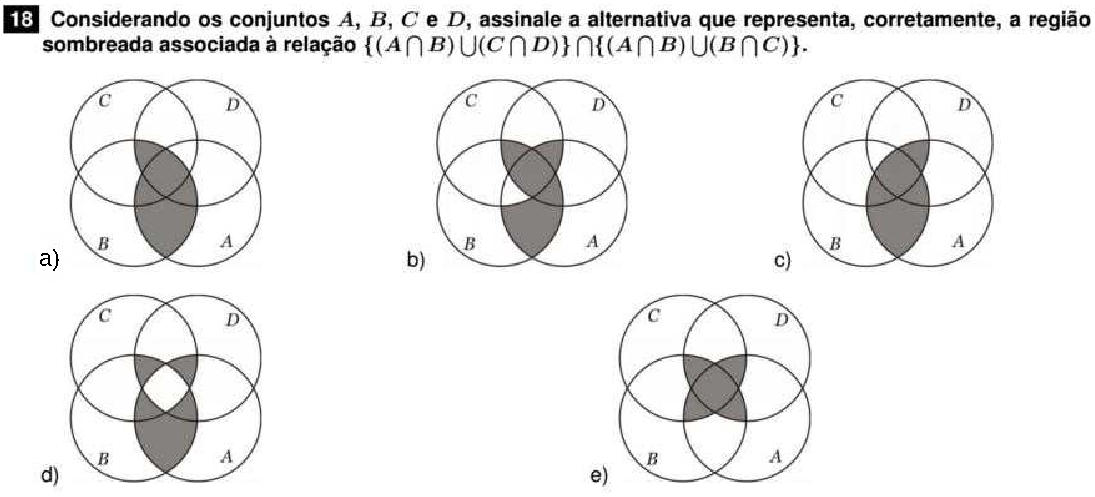
\includegraphics[width=0.9\textwidth]{./figs/poscomp18-cropped.pdf}
\end{figure}
\end{frame}

%39
\begin{frame}{Operações em conjuntos}
    \textbf{Produto cartesiano}: Sejam A e B subconjuntos de S. O produto cartesiano de A e B, denotado por $A \times B$, é definido por

    \[ A \times B = \{(x, y)|x \in A \wedge y \in B\}\]

    \begin{itemize}
        \item Os elementos do resultado não pertencem a S mas são pares ordenados de elementos de S.
        \item O produto $A \times A$ é denotado por $A^2$.
        \item $A^n$ denota o conjunto $(x_1, x_2, ..., x_n)$ de elementos de
        A.
    \end{itemize}

    \textbf{Exemplo:} sejam $A=\{1,2\}$ e $B=\{3,4\}$

    \begin{multicols}{2}
    \begin{enumerate}
        \item Encontre $A \times B$
        \item Encontre $B \times A$
        \item Encontre $A^2$
        \item Encontre $A^3$
    \end{enumerate}
\end{multicols}

\end{frame}

%40
\begin{frame}{Identidades básicas}
    \textbf{Identidades básicas envolvendo conjuntos}: 
    
    \begin{itemize}
        \item Existem várias igualdades entre conjuntos nas operações de união, interseção, diferença e complementação.
        \item Essas igualdades são independentes dos subconjuntos particulares utilizados e são chamadas de identidades.
        \begin{itemize}
            \item Essas identidades são semelhantes às equivalências tautológicas da lógica formal.
        \end{itemize}
    \end{itemize}
\end{frame}

%41
\begin{frame}{Identidades básicas}
    \textbf{Identidades básicas envolvendo conjuntos}: 

    \begin{table}[ht]
        \centering
        \begin{tabular}{|c|c|c|}
        \hline
        \textbf{Propriedade} & \textbf{Identidade 1} & \textbf{Identidade 2} \\ \hline
        Elementos Neutros & 
        $ A \cup \emptyset = A $ & $ A \cap U = A $ \\ \hline
        Dominação & 
        $ A \cup U = U $ & $ A \cap \emptyset = \emptyset $ \\ \hline
        Idempotentes & 
        $ A \cup A = A $ & $ A \cap A = A $ \\ \hline
        Complementação & 
        $ \overline{(\overline{A})} = A $ & - \\ \hline 
        Comutativa & 
        $ A \cup B = B \cup A $ & $ A \cap B = B \cap A $ \\ \hline
        Associativa & 
        $ A \cup (B \cup C) = (A \cup B) \cup C $ & $ A \cap (B \cap C) = (A \cap B) \cap C $ \\ \hline
        Distributiva & 
        $ A \cap (B \cup C) = (A \cap B) \cup (A \cap C) $ & $ A \cup (B \cap C) = (A \cup B) \cap (A \cup C) $ \\ \hline
        De Morgan & 
        $ \overline{A \cup B} = \overline{A} \cap \overline{B} $ & $ \overline{A \cap B} = \overline{A} \cup \overline{B} $ \\ \hline
        Absorção & 
        $ A \cup (A \cap B) = A $ & $ A \cap (A \cup B) = A $ \\ \hline
        \end{tabular}
        \caption{Propriedades e Identidades}
        \end{table}
        

\end{frame}


\begin{frame}{Identidades Básicas}
    \begin{itemize}
        \item \textbf{Provando identidades:} Ex. $A \cup (B \cap C) = (A \cup B) \cap (A \cup C)$
    \end{itemize}

    Queremos então provar que:
    \[
    A \cup (B \cap C) \subseteq (A \cup B) \cap (A \cup C)
    \]
    e que
    \[
    (A \cup B) \cap (A \cup C) \subseteq A \cup (B \cap C)
    \]

    Podemos, então, proceder da seguinte maneira: 
    
    \begin{center}
        (seja $x$ um elemento arbitrário de $A \cup (B \cap C)$):
    \end{center}
    
    \begin{multicols}{2}
        \begin{enumerate}
            \item $x \in A \cup (B \cap C) \rightarrow x \in A$ ou $x \in (B \cap C)$
            \item $\rightarrow x \in A$ ou $(x \in B$ e $x \in C)$
            \item $\rightarrow (x \in A$ ou $x \in B)$ e $(x \in A$ ou $x \in C)$
            \item $\rightarrow x \in (A \cup B)$ e $x \in (A \cup C)$
            \item $\rightarrow x \in (A \cup B) \cap (A \cup C)$
        \end{enumerate}
    \end{multicols}
    
    
    Para mostrarmos que $(A \cup B) \cap (A \cup C) \subseteq A \cup (B \cap C)$, basta fazer o argumento de trás para frente.
\end{frame}

%43
\begin{frame}{Identidades Básicas}
    Ex: Use as identidades básicas para provar que:

\[
[A \cup (B \cap C)] \cap ([\overline{A} \cup (B \cap C)] \cap \overline{(B \cap C)}) = \emptyset
\]

\begin{enumerate}
    \item $\{[A \cup (B \cap C)] \cap (\overline{A} \cup (B \cap C))\} \cap \overline{(B \cap C)}$ \hspace{0.5cm} (associatividade)
    \item $\{[(B \cap C) \cup A] \cap [(B \cap C) \cup \overline{A}]\} \cap \overline{(B \cap C)}$ \hspace{0.5cm} (comutatividade)
    \item $[(B \cap C) \cup (A \cap \overline{A})] \cap \overline{(B \cap C)}$ \hspace{0.5cm} (distributividade)
    \item $[(B \cap C) \cup \emptyset] \cap \overline{(B \cap C)}$ \hspace{0.5cm} (complemento)
    \item $(B \cap C) \cap \overline{(B \cap C)}$ \hspace{0.5cm} (elemento neutro)
    \item $\emptyset$ \hspace{0.5cm} (complemento)
\end{enumerate}
\end{frame}

%44
\begin{frame}{Identidades Básicas}
    Ex: Use as identidades básicas para provar que:

    
\[
    [C \cap (A \cup B)] \cup [(A \cup B) \cap \overline{C}] = (A \cup B)
\]

\pause

\begin{enumerate}
    \item $[(A \cup B) \cap C] \cup [(A \cup B) \cap \overline{C}]$ (comutatividade)
    \item $(A \cup B) \cap (C \cup \overline{C})$ (distributividade)
    \item $(A \cup B) \cap S$ (complemento)
    \item $(A \cup B)$ (elemento neutro)
\end{enumerate}
\end{frame}

\begin{frame}{Identidades Básicas}
\begin{itemize}
    \item A,B e C são subconjuntos de S. Demonstre a seguinte identidade usando as identidades básicas de conjuntos.
\end{itemize}

\[ [A \cap (B \cup C)] \cup ([\overline{A} \cap (B \cup C)] \cup \overline{(B \cup C)}) = S \]
\end{frame}

\begin{frame}{Identidades Básicas}
    \textbf{Identidades envolvendo Conjuntos}

    \begin{itemize}
        \item A,B e C são subconjuntos de S. Demonstre a seguinte identidade usando as identidades básicas de conjuntos.
    \end{itemize}
    
    \[ [A \cap (B \cup C)] \cup ([\overline{A} \cap (B \cup C)] \cup \overline{(B \cup C)}) = S \]
    \end{frame}

    \begin{frame}{Identidades Básicas}
        \textbf{Identidades envolvendo Conjuntos}

        \begin{itemize}
    \item O dual de cada identidade é obtido permutando-se $\cup$
com $\cap$ e $S$ com $\emptyset$. Por exemplo: 

O dual de 

    
    \begin{center}
        $
        [A \cup (B \cap C)] \cap \left([\overline{A} \cup (B \cap C)] \cap \overline{(B \cap C)}\right) = \emptyset
        $ é
        
        $
        [A \cap (B \cup C)] \cup \left([\overline{A} \cap (B \cup C)] \cup \overline{(B \cup C)}\right) = S
        $
    \end{center}
    


\item Essa identidade também pode ser provada substituindo
cada identidade básica pela sua dual.

        \end{itemize}
    \end{frame}


\begin{frame}{Identidades Básicas}
    \begin{itemize}
        \item \textbf{Ex. 1} Usando as identidades básicas, prove a identidade:

            \[
            [C \cap (A \cup B)] \cup \left[(A \cup B) \cap \overline{C}\right] = A \cup B
            \]

            \begin{center}
                (A, B e C são subconjuntos arbitrários de $S$.)
            \end{center}
        \item \textbf{Ex. 2} Enuncie a identidade dual do exemplo anterior.

        \item \textbf{Ex. 3} Usando as identidades básicas, prove a identidade: 
        
        \[
        (A \cup B) \cap (A \cup \overline{B}) = A
        \]
    \end{itemize}
    \end{frame}

\begin{frame}{Resumo}
    Resumo dos métodos para provar identidades envolvendo conjuntos

    \begin{table}
        \centering
        \begin{tabular}{|m{6cm}|m{7cm}|}
        \hline
        \textbf{Método} & \textbf{Comentário} \\ \hline
        Desenhe um diagrama de venn & Não é um bom plano, já que nenhum diagrama vai cobrir todos os casos e não demonstrará a identidade no caso geral. \\ \hline
        Prove a inclusão em cada direção & Tome um elemento arbitrário de um dos termos da identidade e mostre que ele pertence ao outro termo, e reciprocamente. \\ \hline
        Use identidades já demonstradas & Verifique se a forma da expressão é
        exatamente igual à forma da
        identidade que você quer usar. \\ \hline
        \end{tabular}
    \end{table}
\end{frame}

\begin{frame}{Conjuntos enumeráveis e não enumeráveis}
\begin{itemize}
    \item Um conjunto é dito contável, quando podemos contar,
    ou enumerar, todos os seus elementos. Ser contável não
    significa que podemos dizer qual o número total de
    elementos do conjunto; significa que podemos dizer
    “aqui está o primeiro elemento”, “aqui está o segundo
    elemento”, e assim por diante.

    \item \textbf{Todo conjunto finito é contável} pois podemos ordenar
    seus elementos em uma lista como a seguinte, onde
    cada elemento da lista representa um elemento do
    conjunto:
\end{itemize}
    \[ s_1, s_2, s_3, ..., s_n\]

\end{frame}

\begin{frame}{Conjuntos enumeráveis e não enumeráveis}
    \begin{itemize}
        \item Um conjunto infinito também pode ser contável, desde
        que tenhamos uma relação biunívoca com o números
        naturais. Ou seja, podemos relacionar cada elemento
        desse conjunto infinito com um elemento dos números
        naturais.
        \item Um conjunto é dito \textbf{enumerável}, quando for \textbf{infinito e contável}.
    \end{itemize}
    
    \end{frame}

\begin{frame}{Conjuntos enumeráveis e não enumeráveis}

        Para verificar se um conjunto é enumerável precisamos
organizar uma lista de seus elementos.
    
\vspace{2mm}
    \textbf{Exemplos:}

    Verifique que os conjuntos a seguir são enumeráveis:

        \begin{enumerate}
            \item Conjunto dos números ímpares positivos.
            \item Conjunto dos múltiplos de 5.
            \item Conjunto dos números naturais.
            \item Conjuntos dos números inteiros.
        \end{enumerate}
        
    \end{frame}


    \begin{frame}{Conjuntos enumeráveis e não enumeráveis}

        Os conjuntos infinitos que não podem ser enumerados
são não-enumeráveis.
    
\vspace{2mm}
    \textbf{Exemplos:}

        \begin{enumerate}
            \item O conjunto de todos os reais entre 0 e 1.
            \item Um intervalo de números reais.
            \item O conjunto dos números reais.
        \end{enumerate}
        
    \end{frame}
\end{document}